\documentclass[11pt,a4paper]{article}
\usepackage[margin=28mm]{geometry}
\usepackage{amsmath,amssymb,amsthm,mathtools}
\usepackage[round,authoryear]{natbib}
\usepackage[T1]{fontenc}
\usepackage{lmodern}
\usepackage{microtype}
\usepackage{enumitem}
\usepackage{booktabs}
\usepackage{graphicx}
\usepackage[hidelinks]{hyperref}
\hypersetup{pdftitle={Exact reciprocal simplex correlations and their limitations as an earthquake model},pdfsubject={Working manuscript, 19 October 2026}}

\newtheorem{theorem}{Theorem}[section]
\newtheorem{proposition}[theorem]{Proposition}
\newtheorem{lemma}[theorem]{Lemma}
\newtheorem{corollary}[theorem]{Corollary}
\theoremstyle{definition}
\newtheorem{definition}[theorem]{Definition}
\theoremstyle{remark}
\newtheorem{remark}[theorem]{Remark}

\newcommand{\R}{\mathbb R}
\newcommand{\E}{\mathbb E}
\newcommand{\1}{\mathbf 1}
\newcommand{\diam}{\operatorname{diam}}
\newcommand{\vol}{\operatorname{vol}}
\newcommand{\K}{K}
\newcommand{\M}{\mathcal M}
\newcommand{\X}{X}

\title{Exact reciprocal simplex correlations and their limitations as an earthquake model}
\author{}
\date{Draft: 19 October 2026}

\begin{document}
\maketitle

\begin{abstract}
Empirical studies of earthquake catalogues have reported approximate reciprocal dependence on distance for pairs, area for triples, and volume for quadruples. We ask whether one stationary point process can satisfy all three laws as exact full factorial correlations. We construct a simple isotropic finite-cluster process for which the answer is yes on explicit finite distance and shape domains. The construction accounts for every allocation of tuple points to different parents and yields nonnegative cluster densities with the required marginals. We also show why reciprocal tails cannot persist to every scale and why a reciprocal-volume law cannot include unrestricted flattening when fourth local moments are finite. A separate simulation study checks the bounded-window sampler and translation-corrected estimators against the analytical model, while keeping numerical evidence distinct from the proof. The $K$-function and pooled pair and triangle estimates reproduce their targets at the predeclared resolution; only 126 admissible tetrahedra are observed, so the fourth-order estimates remain underpowered. The resulting process is a compatibility witness, not a fitted earthquake model: its intensity is extremely low, it lacks temporal and magnitude dynamics, and a matched comparison with the historical catalogues remains to be done.
\end{abstract}

\section{Introduction}
\label{sec:intro}

Spatial earthquake studies have compared the number of observed pairs, triples and quadruples with the corresponding counts in randomised catalogues. The reported summaries suggest reciprocal dependence on pair distance, triangle area and tetrahedron volume over resolved ranges of scales and shapes \citep{kaganKnopoff1980,kagan1981three,kagan1981four}. These are empirical comparisons of finite catalogues. Their ratios depend on the observation window, the random reference catalogue and the chosen configuration bins; they are not automatically the product densities of a stationary process. The distinction matters when we turn an empirical pattern into a mathematical question. Exercise~12.6.11 of \citet{daleyVereJones2008} asks whether the reciprocal factorial-density forms are compatible and whether fault-based processes can reproduce them approximately. We study the exact question on explicitly restricted domains.

Here we ask whether the three reciprocal forms can hold simultaneously as exact, full correlation identities on specified nontrivial domains. The answer is yes. We construct one simple stationary isotropic process on all of $\R^3$ with positive finite intensity and finite local exponential moments, whose full second-, third- and fourth-order product densities satisfy
\[
 g_2(x_1,x_2)=\frac{C_2}{D},\qquad
 g_3(x_1,x_2,x_3)=\frac{C_3}{A},\qquad
 g_4(x_1,x_2,x_3,x_4)=\frac{C_4}{V}
\]
on finite distance and shape domains. Here $D$ is pair distance, $A$ is triangle area, and $V$ is tetrahedron volume. The constants are positive and fixed across each entire domain.

The exactness concerns the full process. A tuple may use points from several clusters, and all such parent allocations contribute to $g_k$. We first prescribe the full densities and subtract these cross-parent terms. We then recover genuine cluster laws by subtracting the lower-order marginals of clusters of larger sizes. This second step is the delicate one: formal residual kernels would not define a point process unless they were nonnegative and integrable. Explicit geometric bounds and a small but fixed intensity verify those properties.

Point-process realisability has a substantial literature. Kuna, Lebowitz and Speer give low-density realisability results for pair functions and, under additional hard-core and range hypotheses, triplet factors; they also study the realisability problem for pair correlation functions \citep{kunaLebowitzSpeer2007,kunaLebowitzSpeer2011}. These results give context for the cluster construction, but they do not establish the simultaneous reciprocal identities on the restricted pair, triangle and tetrahedron domains proved here.

There are also clear limits to the identities. A full reciprocal-distance law cannot persist to arbitrarily large distances for a stationary process of positive finite intensity. A reciprocal-volume law through arbitrarily flat tetrahedra would force an infinite fourth factorial moment in a bounded window. These obstructions explain two restrictions in our theorem: a finite upper range and a positive lower bound on tetrahedral altitudes. They do not rule out the finite resolved domains used below.

The selected witness uses pair distances from $0.49$ to $50.01$, triangles of diameter at most $36.21$ and least altitude at least $0.49$, and tetrahedra of diameter at most $36.21$ and least vertex-to-opposite-face altitude at least $0.98$, in kilometres. Its intensity is about $1.57\times10^{-9}\,\mathrm{km}^{-3}$. We first establish the exact identities analytically, then check the bounded-window implementation through the three-dimensional $K$-function and full second- to fourth-order estimators. Only after those implementation checks do we return to the earthquake motivation. The historical observation mask has not been recovered, so the present paper does not make a matched catalogue comparison.

\section{Preliminaries}
\label{sec:prelim}

\subsection{Factorial moment measures and product densities}

Let $\X$ be a simple, locally finite point process on $\R^3$. Simplicity means that no location occurs more than once, and local finiteness means that every bounded set contains finitely many points almost surely. For a positive integer $k$, let $\X^k_{\ne}$ denote ordered $k$-tuples of distinct points of $\X$. The $k$th factorial moment measure is defined by
\begin{equation}
 \E\sum_{(x_1,\ldots,x_k)\in\X^k_{\ne}} f(x_1,\ldots,x_k)
 =\int f(x_1,\ldots,x_k)\,\alpha^{(k)}(d x_1\cdots d x_k)
 \label{eq:factorial-measure}
\end{equation}
for nonnegative measurable $f$; see, for example, \citet{daleyVereJones2008}. Distinctness is essential: the vertices of a simplex are different events, and an event cannot fill two vertex positions.

If $\alpha^{(k)}$ is absolutely continuous with respect to $3k$-dimensional Lebesgue measure, its Radon--Nikodym derivative $m_k$ is the (ordered) product density. Thus
\begin{equation}
 \E\sum_{\X^k_{\ne}} f(x_1,\ldots,x_k)
 =\int_{(\R^3)^k} f(x_1,\ldots,x_k)m_k(x_1,\ldots,x_k)\,d x_1\cdots d x_k.
 \label{eq:campbell}
\end{equation}
For disjoint bounded sets $B_1,\ldots,B_k$, the integral of $m_k$ over their product is the expected number of ordered tuples with one point in each set. In a small-region heuristic, $m_k(x_1,\ldots,x_k)$ is the local density of such tuples near the specified locations. Other points elsewhere in the process are unrestricted. This is why $m_k$ is not the density of the event that a specified bounded window contains exactly those $k$ points and no others; that event is described by an exact-configuration or Janossy density.

The integral of $m_k$ over $W^k$ for a bounded $W$ equals the factorial count moment $\E(X(W))_k$, where $(n)_k=n(n-1)\cdots(n-k+1)$. For finite second moments this also gives $\operatorname{Var}X(W)=\rho|W|+\int_{W^2}(m_2(x,y)-\rho^2)\,dx\,dy$ in the stationary case. Existence of a density is a local measure statement and does not by itself imply that all such integrals are finite. We will state moment assumptions separately when they are needed.

\subsection{Normalised correlations}

If the process is stationary with intensity $\rho\in(0,\infty)$, its one-point density is $m_1(x)=\rho$. We use the normalisation
\[
 g_k(x_1,\ldots,x_k)=\frac{m_k(x_1,\ldots,x_k)}{\rho^k}.
\]
This is the stationary version of dividing the product density by the product of the one-point intensities. For a homogeneous Poisson process, $m_k=\rho^k$ and $g_k=1$. A value above one means that tuples near the specified configuration are more frequent than under the Poisson process of the same intensity; a value below one means they are less frequent.

The term \emph{full} distinguishes $g_k$ from connected or factorial-cumulant quantities. At order two the factorial-cumulant density is $m_2-\rho^2$. In the finite-cluster process below, the full densities through order four are sums over all partitions of the tuple according to common parent. The terms from different parents cannot be dropped when claiming an identity for $g_k$.

For an isotropic stationary process in three dimensions, the reduced second-order moment is summarised by
\begin{equation}
 K(r)=4\pi\int_0^r s^2g_2(s)\,ds.
 \label{eq:K-definition}
\end{equation}
The Poisson reference is $K_{\mathrm P}(r)=4\pi r^3/3$. This integrated statistic is useful for checking a sampler and a pair estimator, but it does not determine $g_3$ or $g_4$. We therefore use it as the first, not the final, numerical diagnostic.

\subsection{Simplex geometry and domains}

For two points, write $D=|x_2-x_1|$. For a nondegenerate triangle with vertices $x_1,x_2,x_3$, let $A$ be its area and $d_{\max}$ its longest side. Its least altitude is
\[
 h_3=\frac{2A}{d_{\max}}.
\]
For four affinely independent points, let $V$ be the tetrahedron's volume and let $A_i$ be the area of the face opposite $x_i$. The altitude from $x_i$ to that face is $3V/A_i$; we write $h_4=\min_i3V/A_i$.

Scaling every coordinate by $s>0$ multiplies $D$ and each altitude by $s$, $A$ by $s^2$, and $V$ by $s^3$. Flattening is different: the diameter can stay bounded while a triangle area or tetrahedron volume approaches zero. Our domains control both scale and flattening.

\section{The restricted existence question and its limits}
\label{sec:obstructions}

\subsection{The restricted question}


We ask whether there exist a simple stationary isotropic process on $\R^3$, an intensity $\rho\in(0,\infty)$ and positive constants $C_2,C_3,C_4$ such that its local factorial moments through order four are finite and its full correlations obey $g_2=C_2/D$, $g_3=C_3/A$ and $g_4=C_4/V$ on the domains below. We choose the constants and intensity together as part of the construction; we do not claim to realise arbitrary independently prescribed coefficients.

For positive parameters $\delta,h,H,M,P$, define
\begin{align*}
 S_2&=\{\delta\leq D\leq P\},\\
 S_3&=\{A>0,\ d_{\max}\leq M,\ h_3\geq h\},\\
 S_4&=\{V>0,\ d_{\max}\leq M,\ h_4\geq H\}.
\end{align*}
A sufficient compatibility range is
\begin{equation}
 0<\delta\leq h\leq H<\sqrt{2/3}\,M,\qquad M\leq P<\infty.
 \label{eq:parameter-range}
\end{equation}
The support nesting then holds: each face of a supported tetrahedron is a supported triangle, and each edge of such a triangle is a supported pair. The admissible sets contain open families of different shapes. The theorem below gives the general compatible-domain condition and an explicit witness.

These are domains of correlation identities, not exclusions on all observed configurations. Points from different clusters can form tuples outside them. We first show why removing the upper scale or allowing unrestricted tetrahedral flattening changes the existence question.

\subsection{A reciprocal-distance tail}

\begin{proposition}
\label{prop:pair-tail}
Let $\X$ be stationary and locally finite on $\R^3$, with intensity $0<\rho<\infty$. Suppose its second factorial moment measure has a density on all sufficiently separated pairs. There is no finite $C>0$ such that $g_2(x,y)=C/|x-y|$ for almost every pair at all sufficiently large separations.
\end{proposition}

The contradiction uses only occupancy of separated boxes. A positive intensity gives a fixed positive probability that a bounded box is occupied. If the full pair density decayed as $1/D$, the probability that two far-separated boxes were both occupied would tend to zero. Taking many boxes at increasing separation then contradicts the second-moment inequality $(\E S)^2\leq\E S^2$. Appendix~\ref{app:obstructions} gives the details. The result concerns an infinite-range strengthening and does not contradict observations over a finite range.

\begin{proposition}
\label{prop:higher-tail}
Let $\X$ be stationary with positive finite intensity. A full identity $g_3=C_3/A$ with $C_3>0$ cannot hold on all nondegenerate triangles whose minimum altitude exceeds a fixed positive threshold and whose diameter is unrestricted. The same holds for $g_4=C_4/V$ on all tetrahedra whose minimum vertex altitude exceeds a fixed positive threshold. In each case the density must represent the full factorial moment measure on the stated domain.
\end{proposition}

This higher-order obstruction needs no finite local $k$th moment assumption. The proof places many boxes at dilated centres for which every triple or quadruple is nondegenerate. A reciprocal content density makes the joint occupancy of any $k$ distinct boxes uniformly small, while Jensen's inequality forces the $k$th moment of the total occupancy count to be at least the $k$th power of its mean. Appendix~\ref{app:obstructions} gives the details. The fixed absolute altitude threshold is part of the statement; no claim is made for a scale-invariant shape restriction.

\subsection{Arbitrarily flat tetrahedra}

\begin{proposition}
\label{prop:flat}
Let $\X$ be stationary with intensity $0<\rho<\infty$, a full fourth product density $m_4$, and finite fourth factorial moments on bounded sets. For each noncollinear base $(x_1,x_2,x_3)$, choose orthonormal base-plane vectors $e_1,e_2$ and unit normal $n$. Suppose a domain contains every configuration
\[
 (x_1,x_2,x_3,x_1+s e_1+t e_2+u n),\qquad
 (x_1,x_2,x_3,s,t)\in E,\quad 0<|u|<\epsilon,
\]
where $E$ has positive finite $11$-dimensional Lebesgue measure, is independent of $u$, and its base areas lie between fixed positive finite bounds. Suppose all four vertices lie in one bounded window. Then $g_4=C_4/V$, with $C_4>0$, cannot hold almost everywhere on this family.
\end{proposition}

To see the singularity, fix a base triangle of area $A>0$ and write the fourth vertex in plane coordinates and signed height $u$. Then $V=A|u|/3$. The coordinate Jacobian is a positive constant independent of $u$, so integrating $1/V$ over a set with $u$ near zero includes a positive multiple of $\int_0^\epsilon du/u$. This diverges, whereas the expected number of ordered quadruples in a bounded window is finite. A positive lower altitude removes this singular boundary. The full measure argument appears in Appendix~\ref{app:obstructions}.

\section{A finite-cluster construction}
\label{sec:construction}

We first state a general sufficient condition, then give an explicit witness. Lengths are measured in a fixed unit. Choose
\[
 0<\delta\leq h\leq H<\sqrt{2/3}\,M,\qquad M\leq P<\infty,
\]
with $S_2,S_3,S_4$ as in Section~\ref{sec:obstructions}.

Define the geometric constants
\begin{align}
 I&=2\pi(P^2-\delta^2), & L&=\frac{4\pi}{3}(P^3-\delta^3),\\
 B&=2\pi^2M^2, & C&=6\pi\left[M^2\log(M/H)-\frac{M^2-H^2}{2}\right].
 \label{eq:geom-constants}
\end{align}
Take
\begin{equation}
 a_2=a>0,\qquad
 a_3=\frac{a_2}{4B},\qquad
 a_4=\frac{a_2}{16BC},\qquad
 \rho=a_2I.
 \label{eq:amplitudes}
\end{equation}
The positive scale $a$ is chosen so that the three relative subtraction bounds
\begin{align*}
 E_2&=\frac{\rho^2P}{a_2},\\
 E_3&=\frac{\rho^3M^2}{2a_3}+\frac{3\rho a_2M}{2a_3},\\
 E_4&=\frac{\rho^4M^3}{6a_4}+\frac{\rho^2a_2M^2}{a_4}
       +\frac{a_2^2M}{2a_4}+\frac{4\rho a_3M}{3a_4}
\end{align*}
are at most $1/2$. Such a positive $a$ exists for every compatible choice of geometric parameters: after substitution, each error is a polynomial in $a$ with nonnegative coefficients and zero constant term. The units of $a_2,a_3,a_4,\rho$ are respectively length$^{-5}$, length$^{-7}$, length$^{-9}$ and length$^{-3}$, so $C_k=a_k/\rho^k$ has units length$^{k-1}$.

The construction uses three kinds of density. The target $m_j$ counts all ordered tuples; $q_j$ will count those whose vertices share one parent; and $F_j$ will describe parents emitting exactly $j$ points. For example, a triangle can use three different parents, one pair from a common parent and a third point from another, or a single parent for all three vertices. The respective densities are $\rho^3$, $\rho(q_2(12)+q_2(13)+q_2(23))$, and $q_3(123)$. Subtracting the first two contributions from $a_3/A$ explains the definition of $q_3$ below. The full parent-partition calculation is given in Appendix~\ref{app:partitions}.

For $j=2,3,4$, define $K_2(12)=\1_{S_2}(12)/D(12)$, $K_3(123)=\1_{S_3}(123)/A(123)$ and $K_4(1234)=\1_{S_4}(1234)/V(1234)$, with value zero on degenerate configurations. Define the same-parent kernels successively by
\begin{align}
 q_2(12)&=\1_{S_2}(12)\left(\frac{a_2}{D(12)}-\rho^2\right),\label{eq:q2}\\
 q_3(123)&=\1_{S_3}(123)\left(\frac{a_3}{A(123)}-\rho^3-\rho\sum_{i<j}q_2(ij)\right),\label{eq:q3}\\
 q_4(1234)&=\1_{S_4}(1234)\left(\frac{a_4}{V(1234)}-\rho^4-\rho^2\sum_{i<j}q_2(ij)
 -\sum_{ij|\ell r}q_2(ij)q_2(\ell r)-\rho\sum_{|J|=3}q_3(J)\right).\label{eq:q4}
\end{align}
In the third sum of \eqref{eq:q4}, $ij|\ell r$ runs over the three pairings $12|34$, $13|24$, and $14|23$. The final sum runs over the four triangular faces. Reciprocals are evaluated only on the support indicated by the leading indicator.

A same-parent triangle need not be an entire cluster: it may be three of a four-point cluster's daughters. We must therefore recover the densities for clusters of each exact size from the $q_j$. Let $\M$ denote integration over one omitted point, for example $\M q_4(123)=\int q_4(123z)\,dz$. A four-point cluster contributes $\M F_4$ to the same-parent triangle density and $\tfrac12\M^2F_4$ to the same-parent pair density. Thus
\[
 q_4=F_4,\qquad q_3=F_3+\M F_4,\qquad
 q_2=F_2+\M F_3+\tfrac12\M^2F_4.
\]
The factor $1/2$ accounts for the two orders of the omitted daughters; Appendix~\ref{app:partitions} derives the general multiplicity. Solving these equations from order four downwards gives
\begin{equation}
 F_4=q_4,\qquad F_3=q_3-\M q_4,\qquad
 F_2=q_2-\M q_3+\tfrac12\M^2q_4,
 \label{eq:Fkernels}
\end{equation}
and their anchored normalising constants are
\[
 Z_j=\int F_j(0,y_2,\ldots,y_j)\,dy_2\cdots dy_j,\qquad j=2,3,4.
\]
The kernels are symmetric and translation invariant, so anchoring any coordinate gives the same integral.

\begin{theorem}[Exact reciprocal laws on compatible domains]
\label{thm:main}
For every compatible geometric parameter choice above and every $a>0$ with $E_2,E_3,E_4\leq1/2$, there is a simple stationary isotropic point process $\X$ on $\R^3$ with intensity $\rho=a_2I>0$, finite local exponential moments and infinitely many points almost surely. Its factorial moment measures have ordinary Lebesgue densities at every finite order, and its full densities through order four obey
\begin{align*}
 g_2(12)&=\frac{C_2}{D(12)} && (12\in S_2),\\
 g_3(123)&=\frac{C_3}{A(123)} && (123\in S_3),\\
 g_4(1234)&=\frac{C_4}{V(1234)} && (1234\in S_4),
\end{align*}
where $C_j=a_j/\rho^j$ are positive and fixed on their respective domains. The equalities hold almost everywhere; the explicit density versions in the proof satisfy them at each nondegenerate configuration in the displayed sets. The same construction has independence between restrictions to sets separated by more than $2P$.
\end{theorem}

\begin{proof}
The marginal estimates in Lemma~\ref{lem:marginal-bounds} and the geometric bounds in Lemma~\ref{lem:kernel-positive} imply
\[
 \tfrac12a_jK_j\leq q_j\leq a_jK_j,\qquad
 F_4\geq\tfrac12a_4K_4,\quad F_3\geq\tfrac14a_3K_3,\quad F_2\geq\tfrac14a_2K_2.
\]
All these kernels are finite, have finite anchored integrals and are locally integrable in the full coordinates. In particular $0<Z_j<\infty$. For general compatible parameters, choose a regular tetrahedron of side $s$ with $\sqrt{3/2}\,H<s<M$; its vertex altitudes exceed $H$ and its edges lie below $P$. Small anchored neighbourhoods of this tetrahedron, its faces and its edges have positive measure within the corresponding supports.

Take independent homogeneous Poisson parent processes of types $j=2,3,4$, with rates $Z_j/j!$. A type-$j$ parent at $z$ emits the cluster
\[
 \{z,z+Y_2,\ldots,z+Y_j\},\qquad
 (Y_2,\ldots,Y_j)\text{ has density }F_j(0,\cdot)/Z_j.
\]
Add an independent singleton Poisson process of rate
\begin{equation}
 \lambda_1=\rho^2L+\frac{Z_3}{2}+\frac{Z_4}{3}.
 \label{eq:singleton-rate}
\end{equation}
The bounds above make each cluster mark a probability density. The support cutoffs bound every offset by $P$, and continuous densities give distinct points within clusters. The Poisson parent locations and continuous marks exclude collisions between distinct parents. Only parents in the bounded $P$-enlargement of a bounded observation window can contribute there; their number is finite Poisson and each emits at most four points. Thus the process is simple, locally finite, and has finite local exponential moments. Translation and rotation invariance of the parent laws and kernels give stationarity and isotropy. Since $\lambda_1>0$, the singleton process has infinitely many points almost surely.

We verify the intensity and densities, including all parent allocations. Put $Q_j=\int q_j(0,y_2,\ldots,y_j)\,dy_2\cdots dy_j$. Integrating \eqref{eq:Fkernels} gives
\[
 Z_4=Q_4,\qquad Z_3=Q_3-Q_4,\qquad Z_2=Q_2-Q_3+\tfrac12Q_4,
 \qquad Q_2=a_2I-\rho^2L.
\]
A cluster of size $j$ contributes $Z_j/(j-1)!$ points per unit volume. Hence the non-singleton intensity is $Q_2-Q_3/2+Q_4/6$. Adding \eqref{eq:singleton-rate} gives $Q_2+\rho^2L=\rho$.

For a type-$j$ cluster, its same-parent ordered $r$-tuple density is $\M^{j-r}F_j/(j-r)!$. The factor arises because the parent rate is $Z_j/j!$, the ordered assignment to daughter labels has $j!$ possibilities at full order, and integrating out $j-r$ unobserved daughters counts each ordered $r$-tuple $(j-r)!$ times. Consequently the summed same-parent densities, including singletons, are $\rho,q_2,q_3,q_4$ at orders one through four. Each tuple's parent allocation is a set partition, so the full densities are
\begin{align}
 m_2(12)&=\rho^2+q_2(12),\\
 m_3(123)&=\rho^3+\rho\sum_{i<j}q_2(ij)+q_3(123),\\
 m_4(1234)&=\rho^4+\rho^2\sum_{i<j}q_2(ij)
 +\sum_{ij|\ell r}q_2(ij)q_2(\ell r)+\rho\sum_{|J|=3}q_3(J)+q_4(1234).
 \label{eq:full-partitions}
\end{align}
The Poisson factorial identity for distinct parents proves these formulas as identities of measures; Tonelli's theorem justifies the integrations. Substituting \eqref{eq:q2}--\eqref{eq:q4} cancels every different-parent term on the nested supports and leaves $m_2=a_2/D$, $m_3=a_3/A$ and $m_4=a_4/V$. Division by $\rho^j$ proves the three claims. The parent regions that can influence two sets at distance greater than $2P$ are disjoint, so the restrictions are independent.
\end{proof}

\begin{corollary}[An explicit witness]
With $\delta=h=0.49$, $H=0.98$, $M=36.21$, $P=50.01$ km and $a_2=10^{-13}\,\mathrm{km}^{-5}$, the inequalities $E_j<1/2$ hold. The process in Theorem~\ref{thm:main} has intensity $\rho\approx1.571273848878242\times10^{-9}\,\mathrm{km}^{-3}$ and covers the three expanded domains stated in the introduction.
\end{corollary}

\subsection{A cluster Gibbs representation}
\label{sec:gibbs}

The Poisson construction can also be described by a finite Gibbs law for a single rooted packet. The root is the parent location, which is itself one of the emitted points. This is a representation of the cluster mark; it is not a Gibbs specification for the unlabelled process $\X$.

Merge the four independent parent streams into one marked Poisson process of rate
\[
 \kappa=\lambda_1+Z_2/2!+Z_3/3!+Z_4/4!.
\]
For a packet rooted at the origin, let the anchored reference measure be
\begin{equation}
\nu(d\eta)=\sum_{r=0}^3\frac{\ell_0^{-3r}}{r!}\,du_1\cdots du_r,
 \qquad \eta=\{0,u_1,\ldots,u_r\},
 \label{eq:anchored-reference}
\end{equation}
with the $r=0$ term a unit atom and each integral restricted to distinct offsets in $B(0,P)$. Symmetric functions of the offsets are understood, so the factor $1/r!$ removes their ordering. We take $\ell_0=1$ km and understand each $r$-fold term as $\ell_0^{-3r}\,du_1\cdots du_r$; this makes the reference measure and its densities dimensionless. The density of the packet law with respect to $\nu$ is
\begin{equation}
 w(\{0\})=\frac{\lambda_1}{\kappa},\qquad
 w(\{0\}\cup U)=\frac{\ell_0^{3(j-1)}F_j(0,U)}{j\kappa},\quad |U|=j-1\in\{1,2,3\}.
 \label{eq:gibbs-weight}
\end{equation}
It is zero for packets with more than four points, coincident offsets, or offsets outside the corresponding support. The $1/j$ in \eqref{eq:gibbs-weight} is required: its integral against $\ell_0^{-3(j-1)}dU/(j-1)!$ is $Z_j/(j!\kappa)$, the type-$j$ parent rate divided by $\kappa$. Thus the weights normalise to one.

On the positive support define the finite energy $\mathcal E(\eta)=-\log w(\eta)$; set $\mathcal E=+\infty$ off the support. The hard support and four-point cap are separate constraints. The remaining energy can be written as a sum of rooted interactions of orders two, three and four by Möbius inversion over subsets of the satellites. Every subset of a feasible satellite set is feasible by support nesting, so all weights in the following expression are positive. For a feasible satellite set $U$, put
\[
 E(U)=-\log\frac{w(\{0\}\cup U)}{w(\{0\})},\quad E(\varnothing)=0,
 \qquad \phi(U)=\sum_{B\subseteq U}(-1)^{|U|-|B|}E(B).
\]
Then $E(U)=\sum_{\varnothing\ne B\subseteq U}\phi(B)$. Terms with $|B|=1,2,3$ are respectively the rooted pair, triple and quadruple interactions. This factorisation is exact, but it is only a finite-cluster energy with a distinguished root.

With the convention in \eqref{eq:anchored-reference}, the Papangelou insertion intensity is the ratio of successive densities. For a positive-weight packet with satellite set $U$ and $|U|=r<3$,
\[
\lambda(u;U)=\ell_0^{-3}\frac{w(\{0\}\cup U\cup\{u\})}{w(\{0\}\cup U)}.
\]
It is zero when the insertion violates the support or the size cap. In particular, for an empty satellite set the ratio is $F_2(0,u)/(2\lambda_1)$; for one satellite $v$ it is $2F_3(0,v,u)/(3F_2(0,v))$; and for two satellites $v,w$ it is $3F_4(0,v,w,u)/(4F_3(0,v,w))$. At size four no further insertion is allowed. We use this description to interpret the constructed mark law; no conditional intensity for the entire unlabelled point process is asserted.

\section{Sampling the process in a bounded window}
\label{sec:sampling}

The parent and mark laws above define a whole-space process. To sample its restriction to a bounded observation window $W$, draw every parent that could send at least one point into $W$, including parents outside $W$. Since all offsets have norm at most $P$, parents farther than $P$ from $W$ cannot contribute. The singleton process is sampled directly in $W$.

The normalising constants $Z_j$ need not be evaluated numerically. Appendix~\ref{app:sampler} gives independent Poisson candidate streams whose thinning rates recover the three mark densities exactly. Its proposal distributions have explicit densities, and all acceptance probabilities lie in $[0,1]$ by the positivity bounds already proved. This is an exact probabilistic sampling specification. It does not certify a floating-point implementation or report a simulation comparison.

The sampling order is: generate the finite candidate parent streams on a box containing $W\oplus B(0,P)$; generate the auxiliary geometric proposals and accept or reject each candidate using the stated ratios; retain accepted daughters in $W$; and generate the independent singleton points in $W$. Restricting only parents inside $W$ would be incorrect near the boundary.

\section{Numerical validation of the sampler and correlations}
\label{sec:simulation}

The theorem already establishes the reciprocal identities. The purpose of this study is narrower: to check that the bounded-window sampler and the edge-corrected estimators reproduce the analytical model at the resolution attainable by Monte Carlo. We use the single expanded-witness parameter set
\[
 \delta=h=0.49,\quad H=0.98,\quad M=36.21,\quad P=50.01\ \mathrm{km},
 \qquad a_2=10^{-13}\ \mathrm{km}^{-5}
\]
at every order. It gives
\begin{align*}
 \rho&=1.5712738489\times10^{-9}\ \mathrm{km}^{-3},
 & C_2&=4.05038434\times10^4\ \mathrm{km},\\
 C_3&=2.48998981\times10^8\ \mathrm{km}^2,
 & C_4&=5.15442831\times10^{11}\ \mathrm{km}^3.
\end{align*}
These constants are fixed from the construction; none is fitted to a numerical curve.

\subsection{Design and estimators}

We simulate independent restrictions to equal cubes, including parents outside the observation cube whose daughters can enter it. Every realisation, including empty and low-count cubes, is retained. Parent labels are stored only for sampler diagnostics and are not used by the correlation estimators. The known value of $\rho$ is used throughout the primary study.

The first diagnostic is the translation-corrected estimator of the three-dimensional $K$-function. For the present model,
\begin{equation}
 K(r)=
 \begin{cases}
 4\pi r^3/3,&0\leq r<\delta,\\
 4\pi\delta^3/3+2\pi C_2(r^2-\delta^2),&\delta\leq r\leq P,\\
 4\pi\delta^3/3+2\pi C_2(P^2-\delta^2)+4\pi(r^3-P^3)/3,&r>P.
 \end{cases}
 \label{eq:K-model}
\end{equation}
The curve follows by integrating the full pair correlation; the lower cutoff is not a hard core because points with different parents can be closer than $\delta$. Independent Poisson controls target $4\pi r^3/3$.

We then estimate the full correlations $g_2,g_3,g_4$ with the common translation correction in Appendix~\ref{app:estimators}. Bins lie wholly within their admissible domains. Each estimate is compared with the integrated reciprocal target in \eqref{eq:bin-target}, and the compensated statistics $Dg_2$, $Ag_3$ and $Vg_4$ are compared with the fixed constants above. Table~\ref{tab:frozen-design} records the complete scalar binning and the predeclared shape cuts. Here $d_{\max}$ and $d_{\min}$ are the largest and smallest simplex-edge lengths and $h_{\min}$ is the smallest vertex-to-opposite-face altitude. The orientation variable is $|\cos\theta|$, where $\theta$ is the angle between the vertical axis and the triangle normal or, at fourth order, a longest-edge axis. Each low stratum includes its cut and each high stratum is its complement within the admissible domain. Uncertainty is computed over whole independent realisations.

\begin{table}[htbp]
\centering
\footnotesize
\caption{Frozen numerical design. Scalar edges are in km, km$^2$ and km$^3$
at orders two, three and four. Every adjacent pair defines one bin.}
\label{tab:frozen-design}
\begin{tabular}{@{}lll@{}}
\toprule
Order & scalar-bin edges & shape and orientation cuts\\
\midrule
$g_2$ & \begin{tabular}[t]{@{}l@{}}
$0.49,20.4214,28.8761,35.3641,$\\
$40.8340,45.6531,50.01$
\end{tabular}
& none\\[2pt]
$g_3$ & $0,60.88,128.37,223.24,567.7507$
& \begin{tabular}[t]{@{}l@{}}
$d_{\max}=30.46$ km; $h_{\min}/d_{\max}=0.3281$;\\
$|\cos\theta|=0.5$
\end{tabular}\\[2pt]
$g_4$ & $0,114.32,219.27,465.90,5595.2478$
& \begin{tabular}[t]{@{}l@{}}
$d_{\max}=32.576$ km; $h_{\min}/d_{\max}=0.0954$;\\
$d_{\min}/d_{\max}=0.3327$; $|\cos\theta|=0.5$
\end{tabular}\\
\bottomrule
\end{tabular}
\end{table}

The $K$ grid consists of $0$, $0.245$, $0.49$ km, the multiples of
$10/3$ km from $10/3$ to $100$ km, and the support endpoint $50.01$ km.
At orders three and four, each stratum/bin volume and reciprocal integral is
defined by the integrals in Appendix~\ref{app:estimators} with the corresponding
indicator from Table~\ref{tab:frozen-design}; the independent geometric sampler
uses one million proposals in 50 blocks. Thus the plotted targets do not depend
on undocumented bin midpoints.

\subsection{Precision pilot and fixed production design}

The precision pilot is run before the production design is fixed. It measures runtime, contributing-realisation counts, tuple occupancy, the dispersion of realisation-level contributions, and the uncertainty in the independent geometric normalisers. We use a pointwise 95\% interval half-width no larger than 10\% of the target as a binwise numerical design goal for every pooled bin. This is slightly more demanding than applying the goal only to central bins. A bin that cannot meet it is retained and labelled underpowered; we do not condition on nonempty windows, switch to same-parent tuples, or alter the parameters by order.

The pilot used $10{,}000$ independent cubes of side $1200$ km, seed
$2026101901$, and $250{,}000$ independent geometric proposals at each of orders
three and four. It found $13{,}118$ admissible unordered pairs, $322$ triangles
and only four tetrahedra. The six pair bins met the 10\% pointwise precision
goal, whereas the four pooled triangle bins had relative half-widths between
$20.4\%$ and $24.4\%$. The tetrahedron pilot was plainly uninformative.

We therefore froze the production design before examining its outcomes:
$200{,}000$ independent cubes of the same size, seed $2026101903$, the pilot's
six radial bins and four area and volume bins, and one million independent
geometric proposals per higher order. Pilot scaling predicted useful pair and
triangle estimates but only about 80 admissible tetrahedra. Reaching 10\%
fourth-order precision would require a multi-million-window run, so we retained
the prescribed estimator and recorded fourth order as underpowered. A separate
Poisson control used 200 cubes of side $120$ km at intensity
$3\times10^{-5}\,\mathrm{km}^{-3}$; this deliberately higher intensity checks
the estimators rather than imitating the cluster model.

\subsection{Production results}

The production run retained all $200{,}000$ realisations, including $47{,}055$
empty cubes. Its mean count was $2.71849$, compared with the analytical mean
$2.71516$; the sample variance was $5.32744$. The estimators used every
admissible tuple, without parent labels. For diagnosis only, the saved labels
showed that the $260{,}796$ pairs included 247 two-parent pairs, the $6{,}535$
triangles included 34 two-parent triangles, and the 126 tetrahedra included
three two-parent tetrahedra. Cross-parent allocations are rare at this
intensity, but they were not removed.

\begin{table}[htbp]
\centering
\caption{Production information for the pooled correlation estimates. The
half-width is the largest pointwise 95\% Monte Carlo half-width divided by the
fixed target among the pooled raw and compensated bins.}
\label{tab:simulation-precision}
\begin{tabular}{@{}lrrrl@{}}
\toprule
Order & tuples & scalar bins & largest half-width & assessment\\
\midrule
$g_2$ & $260{,}796$ & 6 & $1.05\%$ & informative\\
$g_3$ & $6{,}535$ & 4 & $5.42\%$ & informative\\
$g_4$ & $126$ & 4 & $39.2\%$ & underpowered\\
\bottomrule
\end{tabular}
\end{table}

The $K$-function follows the analytical curve from the first estimable radius,
$3.33$ km, through $100$ km; the model curve lies in every corresponding
pointwise interval. At $0.245$ and $0.49$ km no pair was observed. The resulting
zero empirical variance is no evidence of precision: at this intensity the
different-parent contribution below the pair support is too rare to estimate.
The higher-intensity Poisson control tracks $4\pi r^3/3$ and supplies the
small-radius implementation check.

\begin{figure}[htbp]
 \centering
 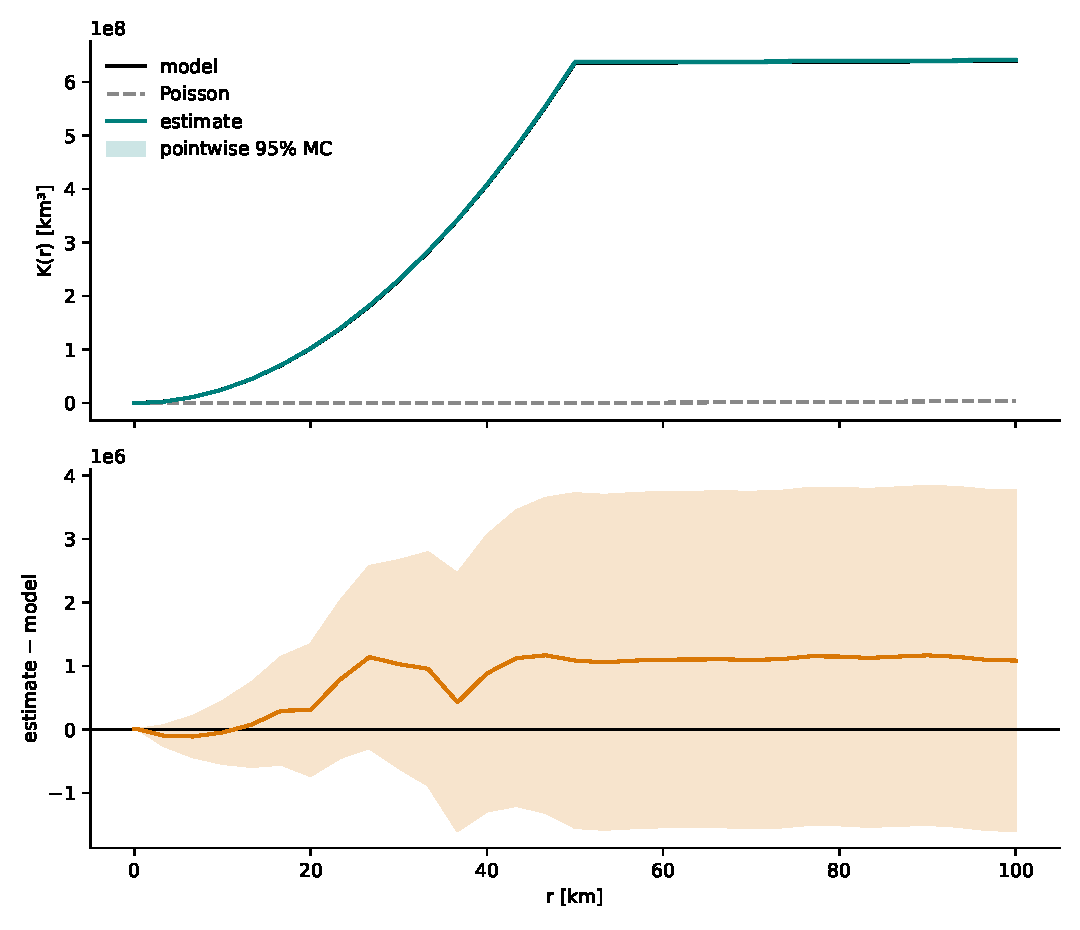
\includegraphics[width=0.83\textwidth]{figures/k_function.pdf}
 \caption{Translation-corrected three-dimensional $K$ estimate, analytical
 model curve and Poisson reference. Shading gives pointwise 95\% Monte Carlo
 intervals over independent realisations.}
 \label{fig:k-check}
\end{figure}

Across the six pair bins, the ratios of estimated to bin-averaged target $g_2$
range from $0.9991$ to $1.0061$. Across the four triangle bins the corresponding
$g_3$ ratios range from $0.9968$ to $1.0203$. Every pair and triangle target
lies in its pointwise interval. The compensated pair ratios range from $0.9995$
to $1.0055$, and the compensated triangle ratios from $0.9889$ to $1.0184$.
The independent geometric normalisers have relative standard errors below
$0.29\%$ for the pooled triangle bins; an independent lower-resolution
normaliser run changed their reciprocal averages by less than $0.44\%$.

\begin{figure}[htbp]
 \centering
 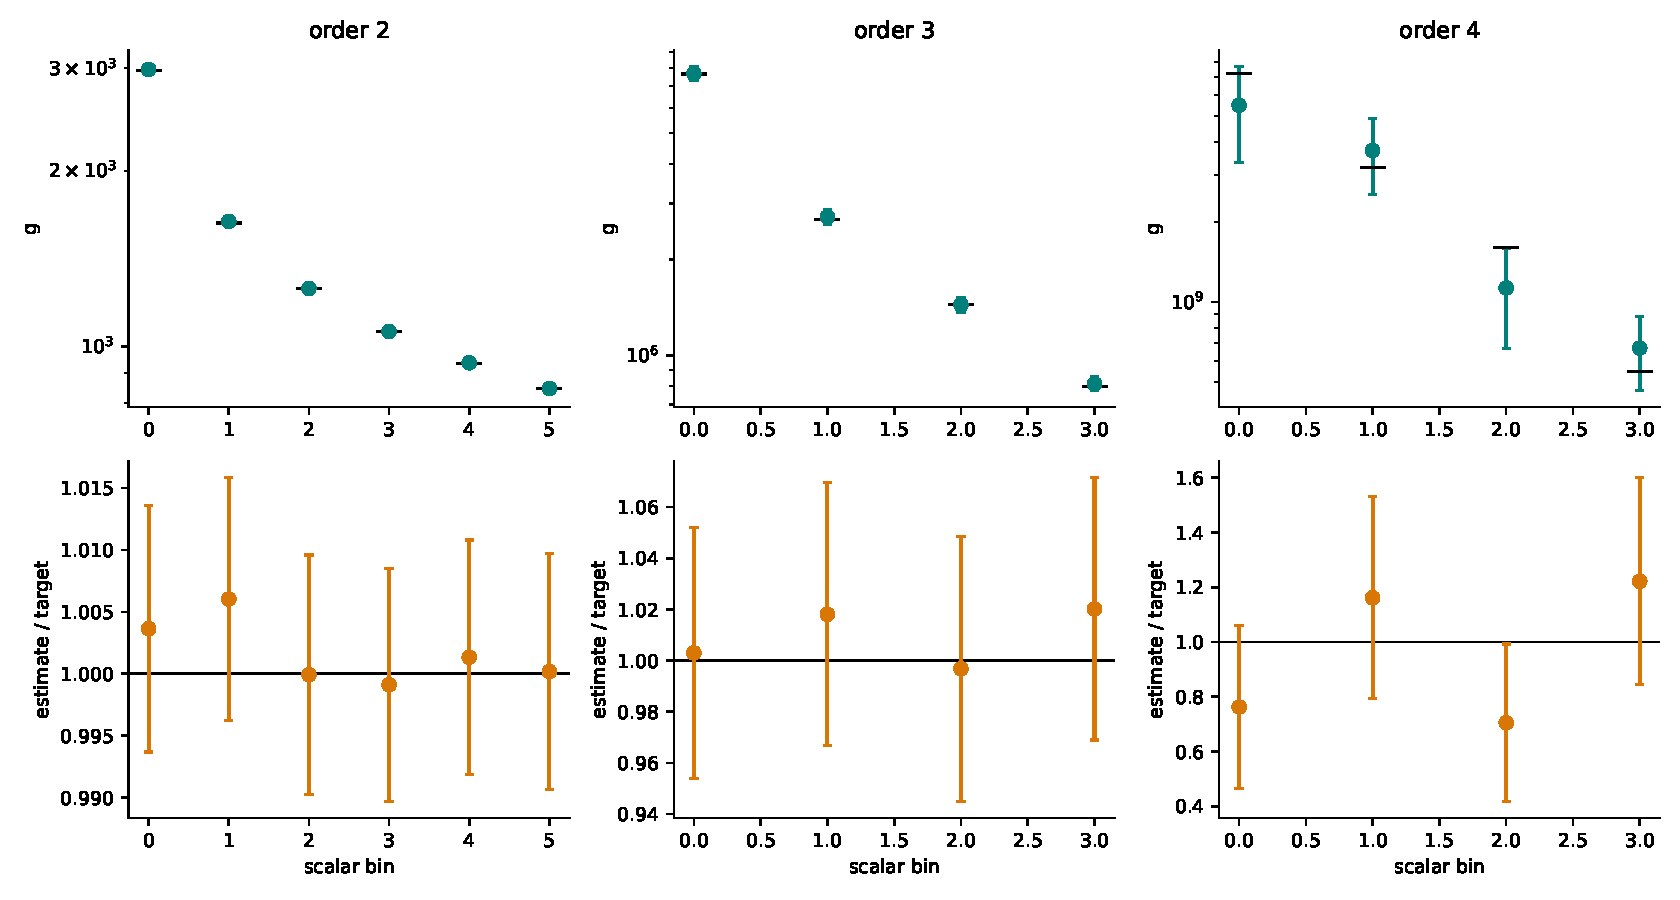
\includegraphics[width=\textwidth]{figures/correlations.pdf}
 \caption{Full correlation estimates against their integrated finite-bin
 reciprocal targets. The lower panels show estimate-to-target ratios. The
 fourth-order intervals are much wider because only 126 admissible
 tetrahedra were observed.}
 \label{fig:correlations}
\end{figure}

\begin{figure}[htbp]
 \centering
 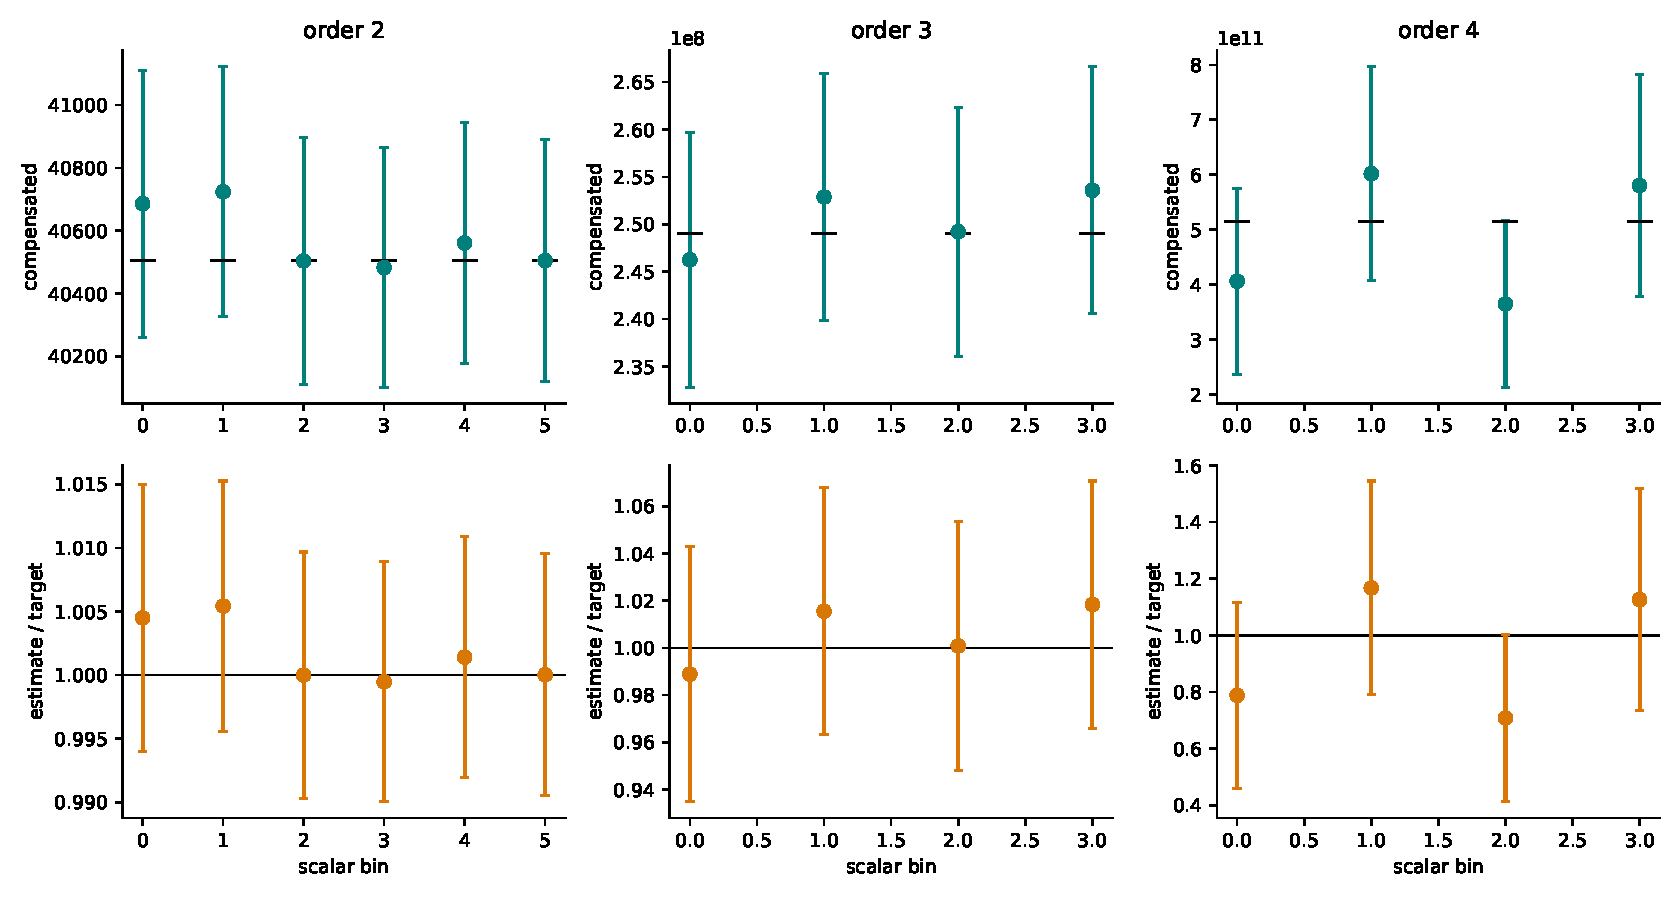
\includegraphics[width=\textwidth]{figures/compensated.pdf}
 \caption{Compensated estimates of $Dg_2$, $Ag_3$ and $Vg_4$ against the fixed
 constants $C_2,C_3,C_4$. Multiplying by the within-tuple geometric quantity,
 rather than a bin midpoint, preserves the exact finite-bin target.}
 \label{fig:compensated}
\end{figure}

Fourth order cannot support the same conclusion. Its four raw ratios are
$0.70$, $0.76$, $1.16$ and $1.22$ after ordering, with relative pointwise
half-widths between $28.8\%$ and $37.9\%$; one raw bin misses its target
interval. All four compensated intervals contain $C_4$, but their half-widths
reach $39.1\%$. The pooled fourth-order normalisers themselves are much more
stable, with relative standard errors below $0.63\%$. The limitation is the
number of observed tetrahedra, not geometric quadrature. These estimates are
inconclusive rather than evidence for or against the analytical identity.

The triangle shape and orientation strata show no resolved systematic
departure: all nonempty compensated intervals contain $C_3$, and the two
orientation groups have estimate-to-target ratios between $0.946$ and $1.069$.
One proposed triangle stratum is geometrically empty and is excluded:
$h_3/d_{\max}\leq0.3281$ implies
$A=d_{\max}h_3/2\leq215.10\,\mathrm{km}^2$, below that bin's lower edge
$223.24\,\mathrm{km}^2$. Fourth-order shape and orientation strata contain
between 0 and 40 tuples per bin and remain underpowered. The independent
normaliser check found no discrepancy larger than $1.82$ joint standard
errors, although one tiny fourth-order stratum changed in volume by $10.8\%$.

\begin{figure}[htbp]
 \centering
 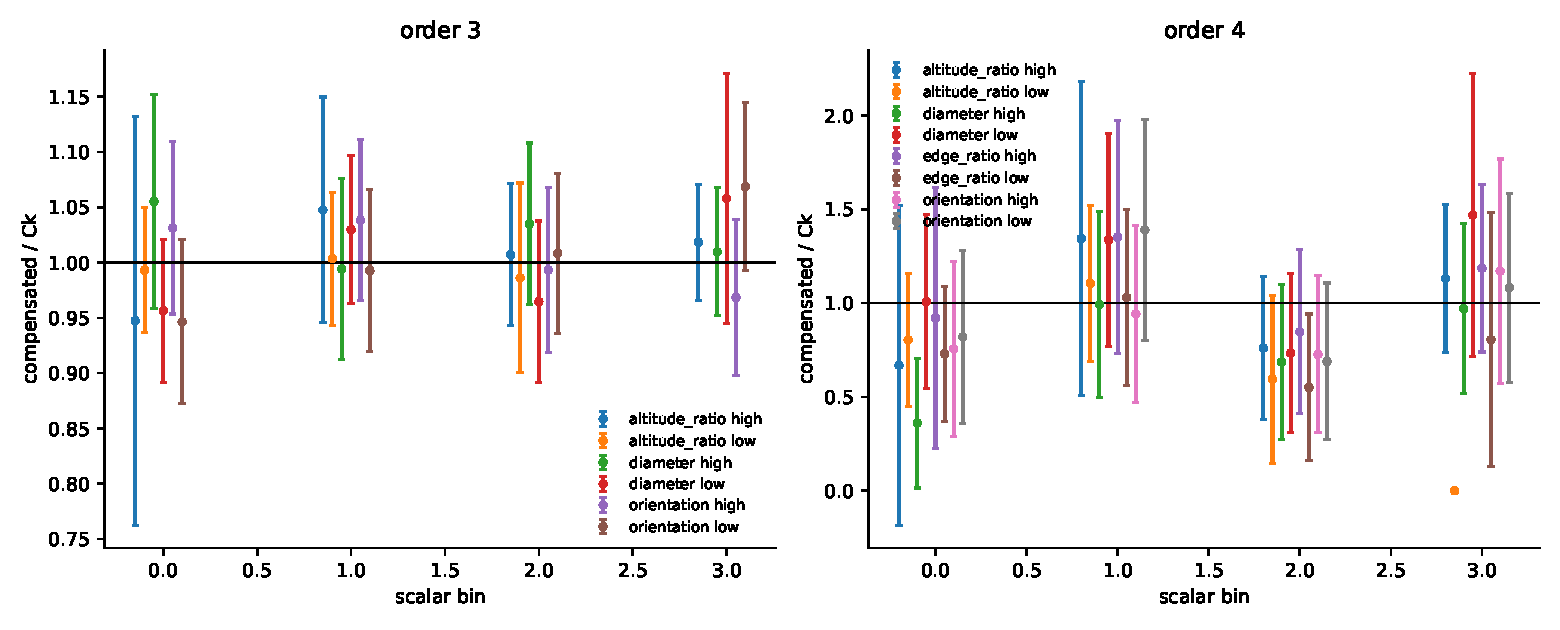
\includegraphics[width=0.9\textwidth]{figures/shape_strata.pdf}
 \caption{Compensated shape and orientation diagnostics. Triangle strata are
 informative except where explicitly sparse or geometrically empty;
 tetrahedron strata are shown to expose, not conceal, their low information.}
 \label{fig:shape-strata}
\end{figure}

Finally, the Poisson controls return correlations close to one at all three
orders. Every pooled Poisson interval contains one: their tuple counts are
$48{,}176$, $17{,}051$ and $7{,}006$ at orders two, three and four. This
separate test supports the ordered-tuple factors, geometric normalisation and
translation correction. It does not repair the sparse fourth-order
cluster-model estimate.

\begin{figure}[htbp]
 \centering
 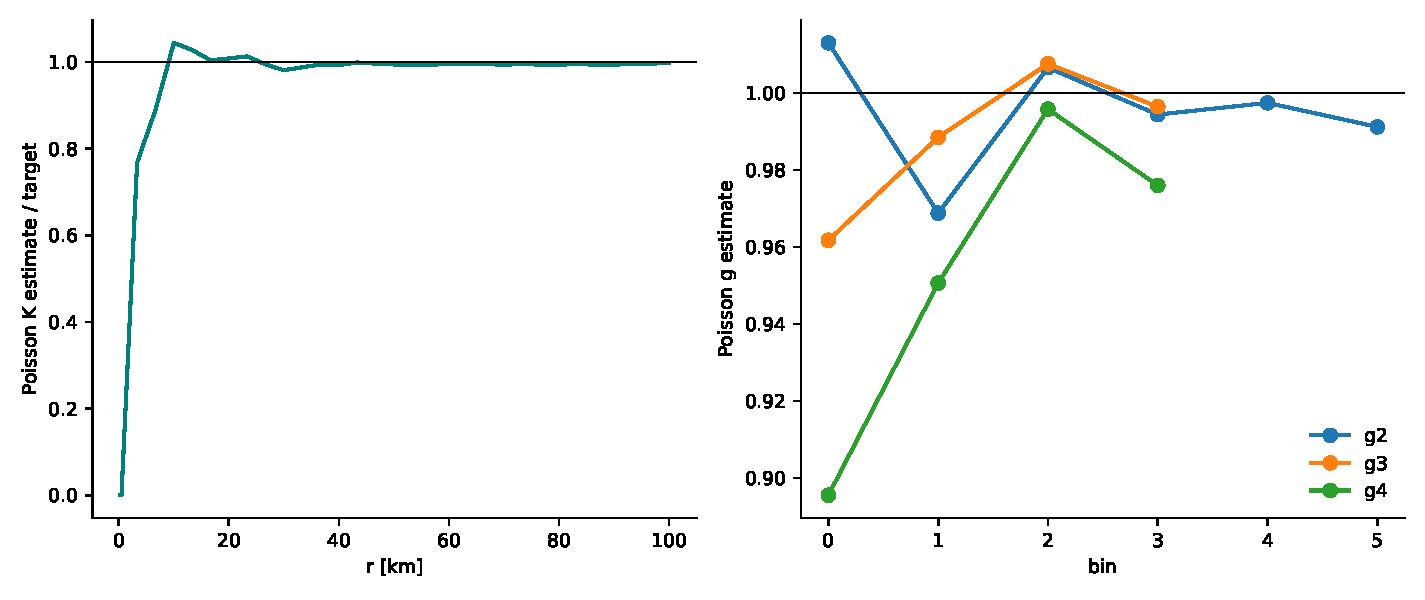
\includegraphics[width=0.85\textwidth]{figures/poisson_controls.pdf}
 \caption{Poisson controls for the $K$ and full-correlation estimators. The
 control intensity is deliberately higher than the witness intensity.}
 \label{fig:poisson-controls}
\end{figure}

All intervals in this section are the pointwise normal intervals defined in
Appendix~\ref{app:estimators}: the relevant mean plus or minus $1.95996$ times
its realisation-level standard error. They are not simultaneous bands or
prediction envelopes. Geometric-normaliser uncertainty is recorded separately
and combined diagnostically, rather than hidden in the realisation-level
standard error.
The normal approximation is particularly rough for the rare fourth-order
contributions and is reported only as a transparent measure of the attained
underpower.
Finite bins and finitely many shape strata do not prove pointwise identities
on a continuum. Their role is to test the implementation against the theorem.

\section{The later earthquake comparison}
\label{sec:earthquake-comparison}

The analytical theorem concerns intrinsic product densities of an ideal stationary process. The numerical study in Section~\ref{sec:simulation} concerns the consistency of a sampler and estimators with that theorem. Neither task by itself compares the model with the finite-catalogue ratios in the earthquake studies. Such a comparison must reproduce the observation window, event selection, location uncertainty, tuple bins and random-reference construction before its ratios can be interpreted.

The required historical observation mask and complete event-selection rule have not yet been recovered. In particular, the illustrative cube of side $378$ km used in earlier count experiments is not an established footprint for the reported $803$-event catalogue. We therefore do not put those counts into the numerical validation study or treat their difference as a fitted-model rejection. The matched earthquake experiment remains planned rather than completed.

When the observation design is available, the comparison should keep three quantities separate: the intrinsic correlation $g_k$, the ratio of expected observed and reference tuple counts, and the expectation of a catalogue-normalised ratio. They agree only under additional conditions. The same study should report count dispersion, empty-window frequency, nearest-neighbour behaviour and shape distributions, since the reciprocal identities constrain only selected factorial correlations. Empty and low-count catalogues must remain in the sample, and one fixed model parameter set must be used at every order.

Even before that comparison, the expanded witness shows an important limitation. Its intensity is approximately $1.5713\times10^{-9}\,\mathrm{km}^{-3}$, so a cube of side $378$ km has expected count about $0.0849$. This calculation describes the witness in an illustrative window; it is not a reconstruction of the historical experiment. A useful earthquake model would also need temporal triggering, magnitude marks, fault geometry and an observation process, none of which is supplied by the present spatial existence construction.

\section{Discussion}
\label{sec:discussion}

The construction answers a compatibility question. It shows that a single stationary, isotropic, simple process can have exact reciprocal full correlations at orders two, three and four on open finite domains. The correlation identities include every allocation of tuple points to different parents. This is the main point of the proof: lower-order residuals must be chosen so that the full densities, rather than only the same-parent contributions, have the required form.

The domain restrictions have separate roles. The finite maximum distance gives finite total integrals for the reciprocal kernels. The positive minimum altitude for tetrahedra keeps the reciprocal-volume kernel integrable in the omitted-vertex direction. The reciprocal-distance kernel is already locally integrable at zero in three dimensions; the lower pair-distance cutoff specifies the resolved support and, together with the triangle altitude cutoff, gives support nesting. These are sufficient features of the construction. The proof does not claim that each cutoff is necessary for every point-process architecture.

The explicit witness has extremely low intensity. This is not an incidental numerical defect in the proof: small amplitudes make the subtractive kernel corrections uniformly small, which certifies positivity. We have not optimised intensity or shown that another finite-cluster law cannot do better. The model also has no time dynamics, magnitude marks, fitted fault geometry or observation process. The finite-range independence is a useful structural property of this witness, but it does not supply these missing earthquake features.

The numerical validation in Section~\ref{sec:simulation} checks a particular sampler and a family of finite-bin estimators; it does not establish the continuum identities, which were proved in Theorem~\ref{thm:main}. The $K$-function and pooled pair and triangle estimates reproduce their targets at useful precision. Fourth order does not: 126 admissible tetrahedra leave every pooled volume bin underpowered. This is a computational consequence of the selected sparse witness, and it also illustrates why an exact existence theorem need not produce an efficient numerical or empirical model. Conversely, exact continuum identities do not determine the finite-catalogue ratios used in the historical studies. Section~\ref{sec:earthquake-comparison} records the observation model still needed for that comparison.

Several questions remain. Can one raise the intensity while preserving all three exact laws and finite local moments? Which broader shape domains admit the same construction? What additional constraints on count distributions or temporal dependence would make a stationary spatial model useful for earthquake catalogues? The present proof supplies one exact starting point for these questions, not their answers.


\appendix
\section{Geometric bounds and positivity}
\label{app:bounds}

This appendix supplies the estimates used in the existence proof. All kernels are zero off their supports, and all integrations below are justified by Tonelli's theorem because the reciprocal kernels are nonnegative.

\begin{lemma}[Marginal bounds]
\label{lem:marginal-bounds}
For the domains in Theorem~\ref{thm:main},
\[
 \M K_3\leq B K_2,\qquad \M K_4\leq C K_3,
\]
where $B,C$ are given in \eqref{eq:geom-constants}.
\end{lemma}

\begin{proof}
Fix a pair at distance $d>0$. Write $r$ for the distance from the omitted vertex to the line through the pair. Its triangle area is $dr/2$. On the support the omitted vertex lies in the ball of radius $M$ about one endpoint, so cylindrical coordinates give
\[
 \int_{B(0,M)}\frac{dz}{r}
 =4\pi\int_0^M\sqrt{M^2-r^2}\,dr=\pi^2M^2.
\]
It follows that $\int K_3(12z)dz\leq 2\pi^2M^2/d=B/d$. If the pair is outside $S_2$, no supported triangle can contain it: each edge of a triangle with least altitude at least $h$ is at least $h\geq\delta$, and its length is at most $M\leq P$. Thus the marginal vanishes there.

Now fix a nondegenerate triangle of area $A$, and write $u$ for signed height of the omitted vertex above its plane. A supported tetrahedron requires $|u|\geq H$ and lies inside the ball of radius $M$ about a base vertex. At height $u$, the in-plane cross-section has area at most $\pi(M^2-u^2)$, and $V=A|u|/3$. Hence
\[
 \int K_4(123z)\,dz
 \leq\frac{6\pi}{A}\int_H^M\frac{M^2-u^2}{u}\,du
 =\frac{C}{A}.
\]
The marginal vanishes outside $S_3$ because each face of a supported tetrahedron is a supported triangle. Indeed, the altitude of a face vertex to an opposite face edge is at least its distance to the tetrahedron face plane, and so is at least $H\geq h$; its edges are at most $M$.
\end{proof}

\begin{lemma}[Pointwise positivity]
\label{lem:kernel-positive}
Write
\begin{align*}
 E_2&=\frac{\rho^2P}{a_2},\\
 E_3&=\frac{\rho^3M^2}{2a_3}+\frac{3\rho a_2M}{2a_3},\\
 E_4&=\frac{\rho^4M^3}{6a_4}+\frac{\rho^2a_2M^2}{a_4}
       +\frac{a_2^2M}{2a_4}+\frac{4\rho a_3M}{3a_4}.
\end{align*}
If $E_j\leq1/2$ for $j=2,3,4$, then
\[
 \frac12a_jK_j\leq q_j\leq a_jK_j,\quad j=2,3,4,
\]
and the actual cluster kernels satisfy
\[
 F_4\geq\frac12a_4K_4,\qquad F_3\geq\frac14a_3K_3,
 \qquad F_2\geq\frac14a_2K_2.
\]
\end{lemma}

\begin{proof}
On $S_2$, multiplying the constant subtraction in $q_2$ by $D/a_2$ gives at most $E_2$. This proves the first pair of bounds. For a triangle of diameter at most $M$, $A\leq M^2/2$ and $A/d\leq M/2$ for every edge $d$. Applying $q_2\leq a_2K_2$ to the three pair terms in $q_3$ bounds the total subtraction relative to $a_3/A$ by $E_3$. Hence the bounds for $q_3$ follow.

For a tetrahedron of diameter at most $M$, determinant and face-area estimates give
\[
 V\leq M^3/6,\quad V/d\leq M^2/6,\quad
 V/(d_{ij}d_{\ell r})\leq M/6,\quad V/A_J\leq M/3.
\]
The third estimate is for disjoint edges. For example,
\[
 6V=|\det(x_2-x_1,x_3-x_1,x_4-x_3)|\leq d_{12}M d_{34};
\]
the other pairings follow by relabelling. Using the already established bounds on $q_2$ and $q_3$ in \eqref{eq:q4}, the six pair terms, three pairings and four faces contribute at most the four terms displayed in $E_4$. This proves the bounds for $q_4$ by induction.

The marginal inequalities now imply
\[
 F_3=q_3-\M q_4\geq(a_3/2-a_4C)K_3=\tfrac14a_3K_3,
\]
since $a_4C=a_3/4$. Also, from \eqref{eq:Fkernels},
\[
 F_2=q_2-\M q_3+\tfrac12\M^2q_4
 \geq (a_2/2-a_3B)K_2=\tfrac14a_2K_2,
\]
since $a_3B=a_2/4$. Finally $F_4=q_4\geq a_4K_4/2$. The alternate expression $F_2=q_2-\M F_3-\frac12\M^2F_4$ gives $F_2\leq q_2$, while $F_3\leq q_3$ follows from its definition. These bounds show finiteness and positivity of every normaliser $Z_j$.
\end{proof}

For the explicit witness, $I<16000$, $B<26000$, $C<110000$, $M<37$ and $P<51$. The first three follow from $\pi<22/7$ and $\log(M/H)<4$; the latter inequality follows from $M/H<37<e^4$. Substitution of \eqref{eq:amplitudes} into the errors gives
\[
 E_2<0.0013056,\qquad E_3<0.009238116,\qquad E_4<0.119547065<\tfrac12.
\]
For clarity, the expressions after substitution are
\begin{align*}
 E_2&=a_2 I^2P,\\
 E_3&=2a_2^2I^3BM^2+6a_2IB M,\\
 E_4&=\tfrac83a_2^3I^4BCM^3+16a_2^2I^2BCM^2
       +8a_2BCM+\tfrac{16}{3}a_2ICM.
\end{align*}
Every coefficient is nonnegative, so these elementary upper bounds certify the continuum positivity inequalities.

\section{Cluster normalisation and parent partitions}
\label{app:partitions}

We justify the same-parent density formula used in Theorem~\ref{thm:main}. A type-$j$ parent at $z$ has relative configuration $\{0,Y_2,\ldots,Y_j\}$ with symmetric density $F_j(0,y_2,\ldots,y_j)/Z_j$ and parent rate $Z_j/j!$. At order $j$, assign an ordered observed tuple to the $j$ labelled daughters in $j!$ ways. The transformation from parent location and offsets to the observed locations has absolute Jacobian one. Reanchoring at whichever observed coordinate is listed first is also a determinant-one linear transformation. Symmetry of $F_j$ therefore gives the full same-parent density $F_j$.

For an ordered $r$-tuple with $r<j$, integrate the $j$-tuple density over the remaining $j-r$ locations. Each specified ordered $r$-tuple is counted $(j-r)!$ times among the assignments of the unobserved daughters. Thus its same-parent density is
\[
 b_r^{(j)}(x_1,\ldots,x_r)
 =\frac1{(j-r)!}\int F_j(x_1,\ldots,x_j)\,dx_{r+1}\cdots dx_j.
\]
The singleton stream contributes $\lambda_1$ at order one. Summing over types and using \eqref{eq:Fkernels} yields $b_1=\rho$, $b_2=q_2$, $b_3=q_3$, and $b_4=q_4$. At orders above four, every nonzero same-parent block has size at most four.

Each ordered tuple has a unique partition of its indices by parent. For distinct Poisson parents, the factorial moment measure is the product of their intensity measures. One can see this first for disjoint bounded parent cells, using independent Poisson counts and $\E(N)_r=\lambda^r$, then extend to nonnegative functions by simple approximation and monotone convergence. A partition with blocks of size at most four contributes the product of the corresponding $b_r$ terms. In particular, at orders two through four the partition sums are exactly \eqref{eq:full-partitions}. This argument is an identity of measures against nonnegative test functions, so it also rules out an omitted singular part in those densities.

The expressions $q_2,q_3,q_4$ are the factorial-cumulant densities of the constructed process: the moment--cumulant partition relations through order four have precisely the forms in \eqref{eq:full-partitions}. The proof of the reciprocal identities only needs the full moment formulas, but this interpretation explains why the recursive subtraction has the form it does.

\section{Proofs of the obstruction statements}
\label{app:obstructions}

\subsection{The pair tail}

Let $B$ be a bounded cube of volume $v>0$, and let $p=\mathbb P\{\X(B)>0\}$. Since $\E\X(B)=\rho v>0$, we have $p>0$. Suppose, for contradiction, that for almost every pair with distance at least $r_0$,
\[
 m_2(x,y)\leq\frac{\rho^2C}{|x-y|}
\]
for a finite $C$. Choose $R>r_0$ so large that $\varepsilon=\rho^2Cv^2/R<p^2/2$. For any integer $n$, take $n$ translates $B_1,\ldots,B_n$ of $B$ with mutual distances at least $R$. Let $I_i=\1\{\X(B_i)>0\}$ and $S_n=\sum_i I_i$. Stationarity gives $\E I_i=p$. For $i\ne j$, disjointness and the second factorial density imply
\[
 \E(I_iI_j)\leq\E[\X(B_i)\X(B_j)]
 =\int_{B_i}\int_{B_j}m_2(x,y)\,dy\,dx\leq\varepsilon.
\]
Consequently,
\[
 n^2p^2=(\E S_n)^2\leq\E S_n^2
 \leq np+n(n-1)\varepsilon.
\]
Divide by $n^2$ and let $n\to\infty$. This gives $p^2\leq\varepsilon<p^2/2$, a contradiction. This proves Proposition~\ref{prop:pair-tail}; the same argument excludes any uniform upper bound $g_2(x,y)\leq b(|x-y|)$ for which $b(r)\to0$.

\subsection{Higher-order reciprocal tails}

The same occupancy idea rules out reciprocal area and volume laws extending to arbitrarily large configurations when the minimum altitudes have fixed positive lower bounds. More precisely, suppose the full $k$th product density is $\rho^k C_k/G_k$ on every $k$-simplex whose relevant altitudes exceed a fixed finite threshold, with no upper diameter bound; here $k=3$ or $4$, and $G_k$ is area or volume. Fix the cube $B$ and its occupancy probability $p>0$ from above, and set $\eta=p^k/2$.

For each $n\geq k$, choose centres $c_i=(i,i^2,i^3)$, $1\leq i\leq n$. Every three centres are noncollinear and every four are affinely independent, by the nonzero Vandermonde determinants of their coordinate projections. For a fixed $n$, take boxes $B_i(T)=Tc_i+B$. As $T\to\infty$, every choice of $k$ points from distinct boxes has simplex content at least a positive constant times $T^{k-1}$, and its nonzero altitudes grow at least linearly in $T$. The bounds are uniform over the boxes because their rescaled points converge uniformly to the finitely many nondegenerate centre tuples. Choose $T=T_n$ large enough that every such tuple lies in the asserted domain and its integrated density over any product of $k$ distinct boxes is at most $\eta$:
\[
 \int_{B_{i_1}(T_n)}\cdots\int_{B_{i_k}(T_n)}m_k(x_1,\ldots,x_k)\,dx_k\cdots dx_1
 \leq \frac{\rho^k C_k v^k}{\inf G_k}\leq\eta.
\]
With $I_i=\1\{\X(B_i(T_n))>0\}$ and $S_n=\sum_iI_i$, each product of $k$ distinct indicators has expectation at most $\eta$. Expand $S_n^k$ into ordered index tuples. There are $(n)_k$ all-distinct tuples; each other term is at most one. By Jensen's inequality and stationarity,
\[
 (np)^k\leq\E S_n^k\leq(n)_k\eta+n^k-(n)_k.
\]
Divide by $n^k$ and let $n\to\infty$. The result $p^k\leq\eta=p^k/2$ is impossible. This higher-order statement concerns an unrestricted upper scale; it is separate from the finite-range tetrahedron obstruction below.

\subsection{The flat-tetrahedron singularity}

Use the family $E$ in Proposition~\ref{prop:flat}. The frame may be chosen measurably by taking $e_1$ along $x_2-x_1$, $n$ in the direction of $(x_2-x_1)\times(x_3-x_1)$ and $e_2=n\times e_1$. For each fixed noncollinear base, the map $(s,t,u)\mapsto x_1+s e_1+t e_2+u n$ preserves three-dimensional Lebesgue measure. Fubini's theorem therefore gives the full four-point volume element $dx_1\,dx_2\,dx_3\,ds\,dt\,du$; variation of the base does not remove any dimensions.

Since $V=A|u|/3$, the integral of $m_4=\rho^4C_4/V$ over this family is
\[
 \left(\int_E\frac{3\rho^4C_4}{A}\,dx_1\,dx_2\,dx_3\,ds\,dt\right)
 \left(\int_{0<|u|<\epsilon}\frac{du}{|u|}\right)=\infty.
\]
The first factor is positive and finite by the area and measure bounds; the second diverges. Tonelli's theorem justifies the factorisation. The integral is bounded above by $\E(X(W))_4$ for the bounded window containing the family, contradicting its finiteness.

In particular, the obstruction applies if a reciprocal-volume law is required for every nondegenerate tetrahedron of diameter below any fixed $M>0$: choose a sufficiently small coplanar square, vary its first three vertices and the fourth vertex's in-plane coordinates over bounded open neighbourhoods with compact closures, and then allow every sufficiently small nonzero height. This provides such a family $E$ while retaining distinct vertices and diameter below $M$. A shape domain whose permitted in-plane sections shrink with the height need not contain this product family; the proposition makes no assertion about that case.

\section{An exact finite-window sampler}
\label{app:sampler}

This appendix specifies a sampler for the exact process without evaluating $Z_2,Z_3,Z_4$ or doing numerical marginal quadrature. All point locations in this algorithm are relative to a candidate parent until acceptance. Reject degenerate geometric proposals, which occur with probability zero.

On $S_j$, put $R_j=q_j/(a_jK_j)$ and set $R_j=0$ off $S_j$. The positivity proof gives $1/2\leq R_j\leq1$ on each support. Let $I_j$ denote its support indicator. For a fixed nondegenerate pair $12$, define a proposal density for a third location by
\[
 Q_3(z\mid12)=\frac{1}{\pi^2M^2\,\operatorname{dist}(z,\operatorname{line}(12))}
 =\frac{D(12)}{B A(12z)},\qquad z\in B(x_1,M).
\]
It integrates to one by the cylindrical calculation in Lemma~\ref{lem:marginal-bounds}. To sample it, decompose $z-x_1$ into coordinate $s$ along the pair line and perpendicular radius $r$. Draw $(s,r)$ uniformly from the half-disc $r\geq0$, $s^2+r^2\leq M^2$, and draw an independent uniform angle.

For a nondegenerate triangle $123$, define
\[
 Q_4(w\mid123)=\frac{3}{C|u|}=\frac{A(123)}{CV(123w)},
 \qquad w\in B(x_1,M),\quad H\leq|u|\leq M,
\]
where $u$ is signed height above the triangle plane. This is also a probability density. One sampler draws $|u|$ log-uniformly on $[H,M]$, accepts with probability $1-u^2/M^2$, chooses the sign fairly, and then chooses the in-plane projection uniformly in the disc of radius $\sqrt{M^2-u^2}$ about $x_1$. Its acceptance probability is positive, so the number of proposals has finite expectation.

Set $J_*=2\pi M^2B$. A proposal with density $1/(J_*A(0,y,z))$ on its full proposal domain can be generated by drawing $y$ with spatial density $1/(2\pi M^2|y|)$ on $0<|y|<M$ and then drawing $z$ from $Q_3(\cdot\mid0,y)$. The joint density is normalised over all nondegenerate pairs $(y,z)$ generated this way, not over $S_3$; configurations outside the required support are rejected. The radial distribution for $y$ is $|y|=M\sqrt U$ with $U$ uniform on $[0,1]$ and direction uniform on the sphere.

Generate the following independent Poisson candidate streams on a bounded box containing $W\oplus B(0,P)$. Candidate locations are uniform in that box conditional on each stream's Poisson count.

\begin{enumerate}[label=\arabic*.]
\item \textbf{Pair parents.} Use candidate rate $a_2I/2$. Draw $Y_2$ with density $K_2(0,y)/I$; equivalently draw a uniform direction and radius $\sqrt{\delta^2+(P^2-\delta^2)U}$. Draw $Z$ from $Q_3(\cdot\mid0,Y_2)$. If $I_3=0$, accept with probability $R_2(0,Y_2)$. If $I_3=1$, also draw $W$ from $Q_4(\cdot\mid0,Y_2,Z)$ and accept with probability
\[
 w_2=R_2-\tfrac14R_3+\tfrac1{32}I_4R_4.
\]
On acceptance emit the parent and its translate by $Y_2$.

\item \textbf{Triple parents.} Use candidate rate $a_3J_*/6$. Draw $Y_2,Y_3$ by the unconditioned proposal above and reject if the triangle is unsupported. Otherwise draw $Y_4$ from $Q_4(\cdot\mid0,Y_2,Y_3)$ and accept with probability
\[
 w_3=R_3-\tfrac14I_4R_4.
\]
On acceptance emit the parent and its two proposed daughters.

\item \textbf{Quadruple parents.} Use candidate rate $a_4J_*C/24$. Draw $Y_2,Y_3$ by the same triangle proposal and then draw $Y_4$ from $Q_4$. Reject unsupported triangles and accept supported tetrahedra with probability $I_4R_4$. On acceptance emit all four points.

\item \textbf{Singleton parents.} Add a direct Poisson process of rate $\rho^2L$. Independently repeat the triangle candidate rule at rate $a_3J_*/2$ and the tetrahedron rule at rate $a_4J_*C/3$, with their same acceptance probabilities, but retain only the parent point and discard proposed daughters.
\end{enumerate}

All acceptance probabilities are valid. For triples, $w_3\geq1/2-1/4=1/4$ on its support and $w_3\leq1$. For pairs with $I_3=1$, $w_2\geq1/2-1/4$ and $w_2\leq1-1/8+1/32<1$; when $I_3=0$, $w_2=R_2$. For quadruples, $I_4R_4\in[0,1]$.

The proposal densities and coefficients $a_3B/a_2=1/4$, $a_4BC/(2a_2)=1/32$, and $a_4C/a_3=1/4$ show that multiplying the candidate rate, proposal density and mean acceptance probability gives marked Poisson intensity density $F_j(0,\cdot)/j!$ per unit parent-location volume. Thus Poisson thinning recovers parent rate $Z_j/j!$ and mark density $F_j/Z_j$. The two auxiliary singleton streams have accepted rates $Z_3/2$ and $Z_4/3$, while the direct stream supplies $\rho^2L$; together they recover \eqref{eq:singleton-rate}. Finally retain emitted points in $W$. Parents outside the chosen $P$-enlargement cannot contribute, so this is the exact restriction of the whole-space process, including boundary-crossing clusters.

\section{Translation-corrected correlation estimators}
\label{app:estimators}

This appendix records the common estimator used in Section~\ref{sec:simulation}. Let $W$ be a rectangular observation box, let $X_b$ be the $b$th of $R$ independent restrictions of the process to $W$, and take the model intensity $\rho$ as known. For an ordered $k$-tuple write $h_1=0$ and $h_i=x_i-x_1$. Its translation overlap is
\[
 v_W(h)=\left|\bigcap_{i=1}^k(W-h_i)\right|.
\]
If the side lengths of $W$ are $L_q$, then
\[
 v_W(h)=\prod_{q=1}^3\left(L_q-\left[\max_i h_{iq}-\min_i h_{iq}\right]\right)_+.
\]

For a relative-configuration bin $B\subset\R^{3(k-1)}$ contained in the relevant admissible domain, define
\begin{equation}
 T_k(B)=\frac{1}{R\rho^k}\sum_{b=1}^R
 \sum_{(x_1,\ldots,x_k)\in X_{b,\ne}^k}
 \frac{\1\{h\in B\}}{v_W(h)}.
 \label{eq:Tk-estimator}
\end{equation}
The change of variables from the tuple to its anchor and relative positions gives
\[
 \E T_k(B)=\int_B g_k(0,h_2,\ldots,h_k)\,dh.
\]
Consequently $T_k(B)/|B|$ estimates the bin average of the full correlation, including tuples whose points have different parents. If unordered tuples are enumerated, the implementation restores the corresponding ordered multiplicity.

Let $G_2=D$, $G_3=A$ and $G_4=V$. The reciprocal target for a finite bin is
\begin{equation}
 \overline g_{k,\mathrm{target}}(B)
 =\frac{C_k}{|B|}\int_B\frac{dh}{G_k(0,h)},
 \label{eq:bin-target}
\end{equation}
not $C_k/G_k$ evaluated at a bin midpoint. The compensated estimator is
\begin{equation}
 \widehat C_k(B)=\frac{1}{R\rho^k|B|}\sum_{b=1}^R
 \sum_{(x_1,\ldots,x_k)\in X_{b,\ne}^k}
 \frac{\1\{h\in B\}G_k(0,h)}{v_W(h)}.
 \label{eq:compensated-estimator}
\end{equation}
Its expectation is exactly $C_k$ for the cluster-model target. Monte Carlo uncertainty is computed over the independent realisations, not over the dependent tuples within a realisation. The geometric bin volumes and reciprocal integrals for orders three and four are evaluated independently of the observed process; their numerical uncertainty is reported with the simulation results.

For completeness, let $Y_b(B)$ denote the $b$th realisation's inner sum in
\eqref{eq:Tk-estimator}, divided by $\rho^k|B|$, and let
\[
 \overline Y=\frac1R\sum_{b=1}^R Y_b,\qquad
 s_Y^2=\frac1{R-1}\sum_{b=1}^R(Y_b-\overline Y)^2.
\]
The displayed raw-correlation interval is
$\overline Y\pm1.95996\,s_Y/\sqrt R$.  The compensated interval uses the same
formula after replacing the inner sum by its $G_k$-weighted version in
\eqref{eq:compensated-estimator}; the $K$ intervals are formed analogously from
one translation-corrected contribution per realisation. Empty realisations
therefore contribute zeros. These are pointwise normal intervals for the mean
estimator, not simultaneous bands. For orders three and four the independent
geometric-normaliser error is tabulated separately and is not folded into
$s_Y/\sqrt R$.


\bibliographystyle{plainnat}
\bibliography{references}
\end{document}
